%Compilation : pdflatex
\documentclass{report}
\makeatletter
\def\@makechapterhead#1{%
  \vspace*{50\p@}%
  {\parindent \z@ \raggedright \normalfont
    \ifnum \c@secnumdepth >\m@ne
      \if@mainmatter
        %\huge\bfseries \@chapapp\space \thechapter
        \Huge\bfseries \thechapter.\space%
        %\par\nobreak
        %\vskip 20\p@
      \fi
    \fi
    \interlinepenalty\@M
    \Huge \bfseries #1\par\nobreak
    \vskip 40\p@
  }}
\makeatother

\usepackage[utf8]{inputenc}
%\usepackage[T1]{fontenc}
\usepackage[a4paper,left=2cm,right=2cm,top=2cm,bottom=2cm]{geometry}
%\usepackage[frenchb]{babel}
%\usepackage{libertine}
\usepackage[pdftex]{graphicx}
\usepackage{color}

%\setlength{\parindent}{0cm}
%\setlength{\parskip}{1ex plus 0.5ex minus 0.2ex}
\newcommand{\hsp}{\hspace{50pt}}
\newcommand{\HRule}{\rule{\linewidth}{0.5mm}}


%\title{Rapport Projet MOGPL}
%\author{Hanane DJEDDAL, Liticia TOUZARI}
%\date{2019-11-24}

%\pagenumbering{gobble} Supprimer numéro de page


\begin{document}
\begin{titlepage}
    \begin{flushleft}
    
\includegraphics[width=11em]{logo.png}\\[1.5cm]
    \end{flushleft}
    %\begin{sffamily}
    \begin{center}
        \textsc{{\LARGE \color{blue} Master Données, Apprentissage et Connaissances-DAC}}\\[5cm]
        \textsc{\Huge{RAPPORT PROJET MOGPL}}\\[1cm]
        \textsc{\Huge{DICE BATTLE}}\\[7cm]
        %\hspace{30pt}
            % Author and supervisor
        \begin{minipage}{1\textwidth}
            \begin{flushleft} \large
            \textsc{\LARGE{Realisé par :}}\\[0.5cm]
            \textsc{Djeddal Hanane}\\
            \textsc{Touzari Liticia}\\
            GROUPE 2\\
            \end{flushleft}
        \end{minipage}
        \vfill
    
        
    \end{center}
   
    
    %\end{sffamily}
  \end{titlepage}
  \tableofcontents
  

  \chapter{Introduction}
  %\addcontentsline{toc}{chapter}{Introduction} \markboth{INTRODUCTION}{} 
  \paragraph{}
  \begin{Large}
  La theorie des jeux est le domaine de mathématique qui permet la modélisation des interactions stratégiques. 
  Dans cet contexte, où plusieurs agents, dites joueurs, cherchent à maximiser leurs gains, le but est de trouver
  une stratégie optimale pour chaque joueur et d'envisager les eventuelles relations liant l'interêt de chauqe 
  joueur, et les possibilités d'un equilibre.\\
  Ce domaine, ayant l'apparence d'un thème restreint, se conforme rapidement à des problèmes d'une grande complexité.\\
  Le but de ce projet est d'etudier les stratégies possibles pour le jeu: Dic-Battle; de comparer expérimentalement ces stratégie
  et à la fin, d'introduire une interface permettant de jouer contre l'ordinateur ou un humain.\\[3.5cm]
  \end{Large}
  \begin{center}
    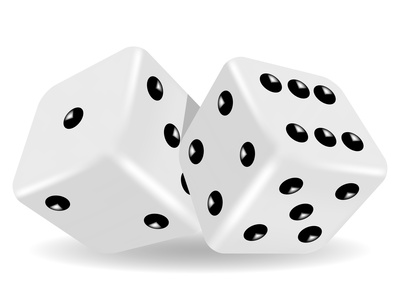
\includegraphics[width=11em]{de.jpg}\\[30cm]
  \end{center}


  \newpage
  \chapter{Description du jeu}
  \paragraph{}
  \begin{large}
  Deux joueurs s'affrontent dans un jeu de dés. Le but est d'être le premier à atteindre au moins
  N points.Le nombre de points marqués est 1 si l'un des dés au moins tombe sur 1,
  dans le cas contraire c'est la somme des dés. On dit qu'un joueur a un gain égal à 1 s'il remporte la partie, un gain égal
  à 0 si la partie est nulle, un gain égal à -1 s'il perd.\\
  Dans ce projet on va étudier deux variante:\\
  - variante séquentielle : les joueurs jouent à tour de rôle;\\
  - variante simultanée : les joueurs jouent simultanément à chaque tour. Dans ce cas si les
  deux joueurs atteignent N points ou plus lors du même tour, c'est le joueur qui dépasse le
  plus les N points qui l'emporte; si les deux joueurs obtiennent le même score, alors ils sont
  ex-aequo.
  \end{large}

  {\let\clearpage\relax \chapter{Probabilite}}   %COPY ME TO ADD A CHAPTER TITLE. :)
  {\let\clearpage\relax \chapter{Variante Séquentielle}} 
  \section{Stratégie aveugle}
  \section{Programmation dynamique}
  \paragraph{}
  \begin{large}
    Dans cette section, on calcule une stratégie en se basant sur la programmation dynamique. Il s'agit 
    de construire une table EG de dimensions (N-1+6D)x(N-1+6D) resprésentant l'éspérance de gain dans un état (i,j) tel que: 
    état(i,j) : état où le premier joueur a cumulé i points, le deuxième joueur a cumulé j
    points, et c'est au joueur 1 de jouer.
    \paragraph{\large{Formule de récurrence: }} \\
    Le jeu étant à somme nulle, l'espérance de gain du joueur 1 est égale à (-) l'espérance de gain de son adversaire. Étant un état (i,j),
    le joueur 2 calcule son espérance de gain, pour un 'd' donné que lance le joueur 1, de la manière suivante:\\
    EG2(j,i)=$\sum_{k=1}^{6d} {P(d,k)EG1(j,i+k)}$ .\\
    Les deux joeurs jouent de façon optimale, la même table est utilisée, et donc le joueur 1 
    est en mesure de calculer EG2 et de joueur de façon à minimiser cet espérance. On aura donc : \\
    EG1(i,j) = - min (EG2(j,i)) = - min($\sum_{k=1}^{6d} {P(d,k)EG(j,i+k)}$) \\
    \underline{Initialisation:}\\
    Si on est dans un état où $i \ge N$ alors soit il a gagné ( $i \ge j$ ), soit il a perdu ( $i \le j$ ), soit la partie est nulle ( i = j ). \\
    $$
\ EG(i,j) = \left\{
    \begin{array}{ll}
        1 & \mbox{si  } i>j, i\ge N \\
        -1 & \mbox{si } i<j, j\ge N  \\
        0 & \mbox{si  } i=j, i\ge N 
    \end{array}
\right.
$$
    \paragraph{\large{La stratégie optimale: }} \\
    Cette approche permet de trouver la stratégie optimale dans chaque état. Il suffit, lors du calcul 
    de l'espérance de gain, de sauvegarder le nombre de dés 'd' permettant d'obtenir ce résultat. 
    \paragraph{\large{Difficulté possible: }}
    Si on supposait que le nombre de points marqués est 0 (et non plus 1) si on obtient au moins un 1, 
    les points cumulés par les joueurs risquent à ne pas changer pendant plusieurs tours. C'est à dire,
    l'algorithme reste dans un état (i,j), et ça pour une durée indéterminée, voir à l'infinie. Donc l'algorithme risque à ne pas se terminer.
    
    \section{Mise en oeuvre}
    \paragraph{\large{Implémentation: }} \\
    \underline{Stratégie aveugle:}\\
    Il s'agit de retourner le 'd' qui maximise la fonction de l'espérance.\\
    \underline{Stratégie optimale:}\\
    En plus de la table EG, la fonction retourne une table 'strat' de même dimension qui donne 
    le nombre de dés optimal à jouer dans chaque état.\\ 
    \underline{Stratégie aléatoire:}\\
    On implémente de plus une stratégie aléatoire qui retoune aléatoirement un nombre entre 1 et D de dés à jouer. \\
    \paragraph{\large{Evaluation: }}\\
    On calcule l'espérance de gain :\\
    \underline{En variant N: } on fixe D à une valeur passée en argument (ici D=10),et pour 
    chaque valeur de N, on simule plusieurs parties et on compte le gain du joueur 1 et joueur 2.\\ 
    
    \subfloat{{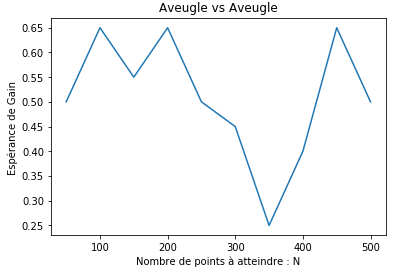
\includegraphics[width=7cm]{Na_a.png} }}%
    \qquad
    \subfloat{{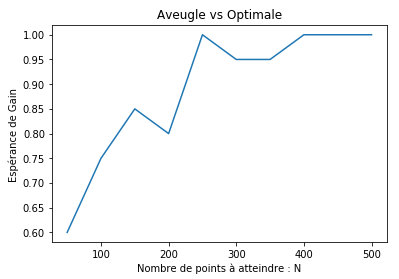
\includegraphics[width=7cm]{Na_o.png} }}%
    \\[1em]
    \subfloat{{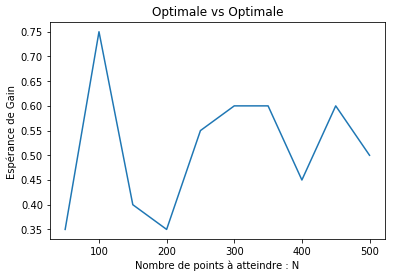
\includegraphics[width=7cm]{No_o.png} }}%
    \qquad
    \subfloat{{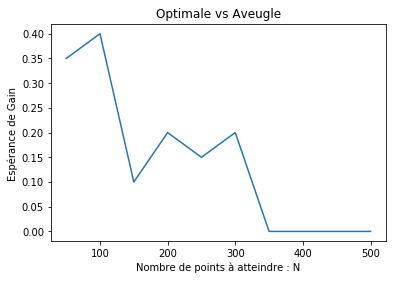
\includegraphics[width=7cm]{No_a.png} }}%
    \\[1em]
    \subfloat{{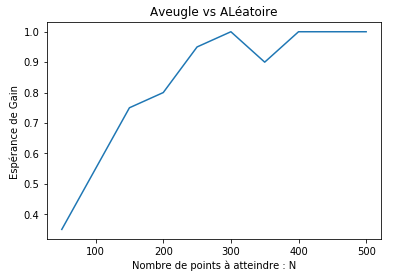
\includegraphics[width=7cm]{Na_r.png} }}%
    \qquad
    \subfloat{{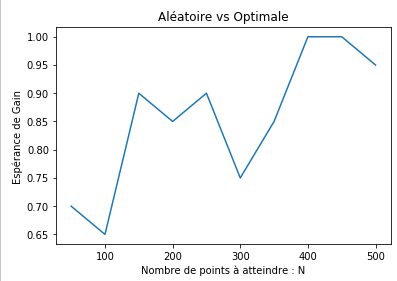
\includegraphics[width=7cm]{Nr_o.png} }}%

    \\[1.5em]
    \underline{En variant D: } on fixe N à une valeur passée en argument (ici N=50),et pour 
    chaque valeur de D, on simule plusieurs parties et on compte le gain du joueur 1 et joueur 2.\\[1.5em]
  
  \end{large}
  

  {\let\clearpage\relax \chapter{Variante Simultanée}} 
  \section{Jeu en un coup}
  \section{Cas général}
  \end{document}
